The client is broken down to different components. The main component for the client will be the Redux state interface, which will keep track of states happening in the application. Other components include logging in as an existing user, registering as a new user, searching through your content once you have connected your accounts from different music platforms, the media player itself, user settings, playlists, oauth, and finally the interface, that will bring it together with the server.

\begin{figure}[h!]
	\centering
 	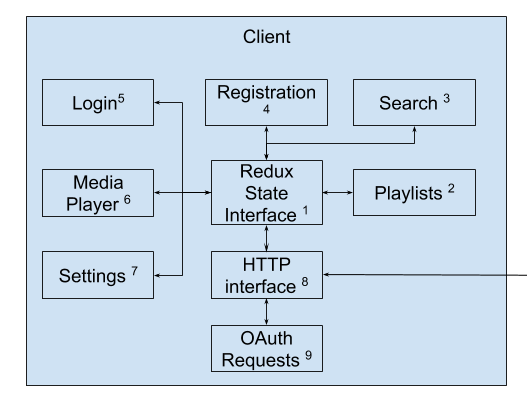
\includegraphics[width=0.60\textwidth]{images/client/ADS-SDS-Client.png}
 	\caption{Client Subsystem}
\end{figure}


\subsection{Layer Hardware}
This layer will require no hardware

\subsection{Layer Operating System}
Chrome 42 and FireFox 39

\subsection{Layer Software Dependencies}
We'll be using React-Redux v6.0.1,  React.js 16.8.0-alpha, The Fetch API from Mozilla, Material-UI v3.9.0, React-Router 4.3

\newpage
